\documentclass[twoside]{book}

% Packages required by doxygen
\usepackage{calc}
\usepackage{doxygen}
\usepackage{graphicx}
\usepackage[utf8]{inputenc}
\usepackage{makeidx}
\usepackage{multicol}
\usepackage{multirow}
\usepackage{fixltx2e}
\PassOptionsToPackage{warn}{textcomp}
\usepackage{textcomp}
\usepackage[nointegrals]{wasysym}
\usepackage[table]{xcolor}

% Font selection
\usepackage[T1]{fontenc}
\usepackage{mathptmx}
\usepackage[scaled=.90]{helvet}
\usepackage{courier}
\usepackage{amssymb}
\usepackage{sectsty}
\renewcommand{\familydefault}{\sfdefault}
\allsectionsfont{%
  \fontseries{bc}\selectfont%
  \color{darkgray}%
}
\renewcommand{\DoxyLabelFont}{%
  \fontseries{bc}\selectfont%
  \color{darkgray}%
}
\newcommand{\+}{\discretionary{\mbox{\scriptsize$\hookleftarrow$}}{}{}}

% Page & text layout
\usepackage{geometry}
\geometry{%
  a4paper,%
  top=2.5cm,%
  bottom=2.5cm,%
  left=2.5cm,%
  right=2.5cm%
}
\tolerance=750
\hfuzz=15pt
\hbadness=750
\setlength{\emergencystretch}{15pt}
\setlength{\parindent}{0cm}
\setlength{\parskip}{0.2cm}
\makeatletter
\renewcommand{\paragraph}{%
  \@startsection{paragraph}{4}{0ex}{-1.0ex}{1.0ex}{%
    \normalfont\normalsize\bfseries\SS@parafont%
  }%
}
\renewcommand{\subparagraph}{%
  \@startsection{subparagraph}{5}{0ex}{-1.0ex}{1.0ex}{%
    \normalfont\normalsize\bfseries\SS@subparafont%
  }%
}
\makeatother

% Headers & footers
\usepackage{fancyhdr}
\pagestyle{fancyplain}
\fancyhead[LE]{\fancyplain{}{\bfseries\thepage}}
\fancyhead[CE]{\fancyplain{}{}}
\fancyhead[RE]{\fancyplain{}{\bfseries\leftmark}}
\fancyhead[LO]{\fancyplain{}{\bfseries\rightmark}}
\fancyhead[CO]{\fancyplain{}{}}
\fancyhead[RO]{\fancyplain{}{\bfseries\thepage}}
\fancyfoot[LE]{\fancyplain{}{}}
\fancyfoot[CE]{\fancyplain{}{}}
\fancyfoot[RE]{\fancyplain{}{\bfseries\scriptsize Generated on Mon Jun 16 2014 14\+:09\+:27 for My Project by Doxygen }}
\fancyfoot[LO]{\fancyplain{}{\bfseries\scriptsize Generated on Mon Jun 16 2014 14\+:09\+:27 for My Project by Doxygen }}
\fancyfoot[CO]{\fancyplain{}{}}
\fancyfoot[RO]{\fancyplain{}{}}
\renewcommand{\footrulewidth}{0.4pt}
\renewcommand{\chaptermark}[1]{%
  \markboth{#1}{}%
}
\renewcommand{\sectionmark}[1]{%
  \markright{\thesection\ #1}%
}

% Indices & bibliography
\usepackage{natbib}
\usepackage[titles]{tocloft}
\setcounter{tocdepth}{3}
\setcounter{secnumdepth}{5}
\makeindex

% Hyperlinks (required, but should be loaded last)
\usepackage{ifpdf}
\ifpdf
  \usepackage[pdftex,pagebackref=true]{hyperref}
\else
  \usepackage[ps2pdf,pagebackref=true]{hyperref}
\fi
\hypersetup{%
  colorlinks=true,%
  linkcolor=blue,%
  citecolor=blue,%
  unicode%
}

% Custom commands
\newcommand{\clearemptydoublepage}{%
  \newpage{\pagestyle{empty}\cleardoublepage}%
}


%===== C O N T E N T S =====

\begin{document}

% Titlepage & ToC
\hypersetup{pageanchor=false,
             bookmarks=true,
             bookmarksnumbered=true,
             pdfencoding=unicode
            }
\pagenumbering{roman}
\begin{titlepage}
\vspace*{7cm}
\begin{center}%
{\Large My Project }\\
\vspace*{1cm}
{\large Generated by Doxygen 1.8.7}\\
\vspace*{0.5cm}
{\small Mon Jun 16 2014 14:09:27}\\
\end{center}
\end{titlepage}
\clearemptydoublepage
\tableofcontents
\clearemptydoublepage
\pagenumbering{arabic}
\hypersetup{pageanchor=true}

%--- Begin generated contents ---
\chapter{Hierarchical Index}
\section{Class Hierarchy}
This inheritance list is sorted roughly, but not completely, alphabetically\+:\begin{DoxyCompactList}
\item \contentsline{section}{bernstein\+\_\+hasher}{\pageref{classbernstein__hasher}}{}
\item \contentsline{section}{suffix\+\_\+trie\+:\+:edge}{\pageref{classsuffix__trie_1_1edge}}{}
\item \contentsline{section}{suffix\+\_\+tree\+:\+:edge}{\pageref{classsuffix__tree_1_1edge}}{}
\item \contentsline{section}{edit\+\_\+distance}{\pageref{classedit__distance}}{}
\item \contentsline{section}{suffix\+\_\+trie\+:\+:node}{\pageref{classsuffix__trie_1_1node}}{}
\item \contentsline{section}{suffix\+\_\+tree\+:\+:node}{\pageref{classsuffix__tree_1_1node}}{}
\item \contentsline{section}{rabin\+\_\+karp\+\_\+searcher}{\pageref{classrabin__karp__searcher}}{}
\item \contentsline{section}{suffix\+\_\+tree}{\pageref{classsuffix__tree}}{}
\item \contentsline{section}{suffix\+\_\+tree\+\_\+builder}{\pageref{classsuffix__tree__builder}}{}
\begin{DoxyCompactList}
\item \contentsline{section}{naive\+\_\+suffix\+\_\+tree\+\_\+builder}{\pageref{classnaive__suffix__tree__builder}}{}
\item \contentsline{section}{ukkonen\+\_\+suffix\+\_\+tree\+\_\+builder}{\pageref{classukkonen__suffix__tree__builder}}{}
\end{DoxyCompactList}
\item \contentsline{section}{suffix\+\_\+trie}{\pageref{classsuffix__trie}}{}
\item \contentsline{section}{suffix\+\_\+trie\+\_\+builder}{\pageref{classsuffix__trie__builder}}{}
\end{DoxyCompactList}

\chapter{Class Index}
\section{Class List}
Here are the classes, structs, unions and interfaces with brief descriptions\+:\begin{DoxyCompactList}
\item\contentsline{section}{\hyperlink{classbernstein__hasher}{bernstein\+\_\+hasher} }{\pageref{classbernstein__hasher}}{}
\item\contentsline{section}{\hyperlink{classedit__distance}{edit\+\_\+distance} }{\pageref{classedit__distance}}{}
\item\contentsline{section}{\hyperlink{classrabin__karp__searcher}{rabin\+\_\+karp\+\_\+searcher} }{\pageref{classrabin__karp__searcher}}{}
\end{DoxyCompactList}

\chapter{File Index}
\section{File List}
Here is a list of all documented files with brief descriptions\+:\begin{DoxyCompactList}
\item\contentsline{section}{\hyperlink{constants_8hpp}{constants.\+hpp} }{\pageref{constants_8hpp}}{}
\item\contentsline{section}{{\bfseries friends.\+hpp} }{\pageref{friends_8hpp}}{}
\item\contentsline{section}{{\bfseries string\+\_\+slib.\+hpp} }{\pageref{string__slib_8hpp}}{}
\item\contentsline{section}{algorithms/\hyperlink{edit__distance_8hpp}{edit\+\_\+distance.\+hpp} }{\pageref{edit__distance_8hpp}}{}
\item\contentsline{section}{algorithms/{\bfseries knuth\+\_\+morris\+\_\+pratt.\+hpp} }{\pageref{algorithms_2knuth__morris__pratt_8hpp}}{}
\item\contentsline{section}{algorithms/\hyperlink{naive_8hpp}{naive.\+hpp} }{\pageref{naive_8hpp}}{}
\item\contentsline{section}{algorithms/\hyperlink{rabin__karp_8hpp}{rabin\+\_\+karp.\+hpp} }{\pageref{rabin__karp_8hpp}}{}
\item\contentsline{section}{algorithms/\hyperlink{z__algorithm_8hpp}{z\+\_\+algorithm.\+hpp} }{\pageref{z__algorithm_8hpp}}{}
\item\contentsline{section}{algorithms/hashing/{\bfseries bernstein.\+hpp} }{\pageref{bernstein_8hpp}}{}
\item\contentsline{section}{algorithms/hashing/{\bfseries hashing.\+hpp} }{\pageref{hashing_8hpp}}{}
\item\contentsline{section}{algorithms/hashing/{\bfseries sum\+\_\+hashing.\+hpp} }{\pageref{sum__hashing_8hpp}}{}
\item\contentsline{section}{structures/{\bfseries knuth\+\_\+morris\+\_\+pratt.\+hpp} }{\pageref{structures_2knuth__morris__pratt_8hpp}}{}
\item\contentsline{section}{structures/{\bfseries suffix\+\_\+tree.\+hpp} }{\pageref{suffix__tree_8hpp}}{}
\end{DoxyCompactList}

\chapter{Class Documentation}
\hypertarget{classbernstein__hasher}{\section{bernstein\+\_\+hasher Class Reference}
\label{classbernstein__hasher}\index{bernstein\+\_\+hasher@{bernstein\+\_\+hasher}}
}
\subsection*{Public Member Functions}
\begin{DoxyCompactItemize}
\item 
\hypertarget{classbernstein__hasher_a3000e6b57d1d8b1aa1e7eab364393b7a}{{\bfseries bernstein\+\_\+hasher} (int base=33, int maximum\+\_\+needle\+\_\+length=1000)}\label{classbernstein__hasher_a3000e6b57d1d8b1aa1e7eab364393b7a}

\item 
\hypertarget{classbernstein__hasher_a0fdc166f2b194fb7531482ad2c9c9a3b}{long long {\bfseries bernstein\+\_\+hash} (const string \&str)}\label{classbernstein__hasher_a0fdc166f2b194fb7531482ad2c9c9a3b}

\item 
\hypertarget{classbernstein__hasher_a629ebbbf40151d70e80a23cf497fbff0}{long long {\bfseries bernstein\+\_\+hash} (const char $\ast$str, int length=-\/1)}\label{classbernstein__hasher_a629ebbbf40151d70e80a23cf497fbff0}

\item 
\hypertarget{classbernstein__hasher_a35677897233e3b7a2556adcb1cc15fbb}{long long {\bfseries next\+\_\+bernstein\+\_\+hash} (const char $\ast$str, int index, long long current\+\_\+hash)}\label{classbernstein__hasher_a35677897233e3b7a2556adcb1cc15fbb}

\item 
\hypertarget{classbernstein__hasher_ab83ee23ba9930624fcf7ec0ecc856fea}{long long {\bfseries remove\+\_\+prefix\+\_\+from\+\_\+hash} (const char $\ast$str, int index, int length, long long current\+\_\+hash)}\label{classbernstein__hasher_ab83ee23ba9930624fcf7ec0ecc856fea}

\end{DoxyCompactItemize}
\subsection*{Static Public Attributes}
\begin{DoxyCompactItemize}
\item 
\hypertarget{classbernstein__hasher_a25a1b74eba73eef405ee6c2ced22e357}{static const int {\bfseries M\+O\+D} =101}\label{classbernstein__hasher_a25a1b74eba73eef405ee6c2ced22e357}

\end{DoxyCompactItemize}


The documentation for this class was generated from the following files\+:\begin{DoxyCompactItemize}
\item 
algorithms/hashing/bernstein.\+hpp\item 
algorithms/hashing/bernstein.\+cpp\end{DoxyCompactItemize}

\hypertarget{classsuffix__trie_1_1edge}{\section{suffix\+\_\+trie\+:\+:edge Class Reference}
\label{classsuffix__trie_1_1edge}\index{suffix\+\_\+trie\+::edge@{suffix\+\_\+trie\+::edge}}
}


{\ttfamily \#include $<$suffix\+\_\+trie.\+hpp$>$}

\subsection*{Public Member Functions}
\begin{DoxyCompactItemize}
\item 
void \hyperlink{classsuffix__trie_1_1edge_a680b647d002f8bcc652e1c018f0c657b}{add\+\_\+index} (int index)
\item 
\hyperlink{classsuffix__trie_1_1edge_aa6f56affb895ee66dc772945a6ebb5ff}{edge} (\hyperlink{classsuffix__trie_1_1node}{suffix\+\_\+trie\+::node} $\ast$\hyperlink{classsuffix__trie_1_1edge_ae89e6815dd581516c8d4284814334263}{from}, \hyperlink{classsuffix__trie_1_1node}{suffix\+\_\+trie\+::node} $\ast$\hyperlink{classsuffix__trie_1_1edge_a356e813f739d3559b031bdcb6da6da76}{to})
\item 
\hyperlink{classsuffix__trie_1_1edge_a10c602847a0349ea05d7aff29493d4e7}{$\sim$edge} ()
\end{DoxyCompactItemize}
\subsection*{Public Attributes}
\begin{DoxyCompactItemize}
\item 
vector$<$ int $>$ \hyperlink{classsuffix__trie_1_1edge_ac5864e7428c08ec02d50039a5dd4eaa6}{s\+\_\+index}
\item 
\hyperlink{classsuffix__trie_1_1node}{suffix\+\_\+trie\+::node} $\ast$ \hyperlink{classsuffix__trie_1_1edge_ae89e6815dd581516c8d4284814334263}{from}
\item 
\hyperlink{classsuffix__trie_1_1node}{suffix\+\_\+trie\+::node} $\ast$ \hyperlink{classsuffix__trie_1_1edge_a356e813f739d3559b031bdcb6da6da76}{to}
\end{DoxyCompactItemize}


\subsection{Detailed Description}
{\itshape \hyperlink{classsuffix__trie_1_1edge}{suffix\+\_\+trie\+::edge}} is an edge in the trie. 

\subsection{Constructor \& Destructor Documentation}
\hypertarget{classsuffix__trie_1_1edge_aa6f56affb895ee66dc772945a6ebb5ff}{\index{suffix\+\_\+trie\+::edge@{suffix\+\_\+trie\+::edge}!edge@{edge}}
\index{edge@{edge}!suffix\+\_\+trie\+::edge@{suffix\+\_\+trie\+::edge}}
\subsubsection[{edge}]{\setlength{\rightskip}{0pt plus 5cm}suffix\+\_\+trie\+::edge\+::edge (
\begin{DoxyParamCaption}
\item[{{\bf suffix\+\_\+trie\+::node} $\ast$}]{from, }
\item[{{\bf suffix\+\_\+trie\+::node} $\ast$}]{to}
\end{DoxyParamCaption}
)}}\label{classsuffix__trie_1_1edge_aa6f56affb895ee66dc772945a6ebb5ff}
creates a {\itshape \hyperlink{classsuffix__trie_1_1edge}{suffix\+\_\+trie\+::edge}} with a given starting {\itshape node} and ending {\itshape node} \hypertarget{classsuffix__trie_1_1edge_a10c602847a0349ea05d7aff29493d4e7}{\index{suffix\+\_\+trie\+::edge@{suffix\+\_\+trie\+::edge}!````~edge@{$\sim$edge}}
\index{````~edge@{$\sim$edge}!suffix\+\_\+trie\+::edge@{suffix\+\_\+trie\+::edge}}
\subsubsection[{$\sim$edge}]{\setlength{\rightskip}{0pt plus 5cm}suffix\+\_\+trie\+::edge\+::$\sim$edge (
\begin{DoxyParamCaption}
{}
\end{DoxyParamCaption}
)}}\label{classsuffix__trie_1_1edge_a10c602847a0349ea05d7aff29493d4e7}
destroys the edge and the outgoing node recursively 

\subsection{Member Function Documentation}
\hypertarget{classsuffix__trie_1_1edge_a680b647d002f8bcc652e1c018f0c657b}{\index{suffix\+\_\+trie\+::edge@{suffix\+\_\+trie\+::edge}!add\+\_\+index@{add\+\_\+index}}
\index{add\+\_\+index@{add\+\_\+index}!suffix\+\_\+trie\+::edge@{suffix\+\_\+trie\+::edge}}
\subsubsection[{add\+\_\+index}]{\setlength{\rightskip}{0pt plus 5cm}void suffix\+\_\+trie\+::edge\+::add\+\_\+index (
\begin{DoxyParamCaption}
\item[{int}]{index}
\end{DoxyParamCaption}
)}}\label{classsuffix__trie_1_1edge_a680b647d002f8bcc652e1c018f0c657b}
adds a new {\itshape index} to {\itshape s\+\_\+index} 

\subsection{Member Data Documentation}
\hypertarget{classsuffix__trie_1_1edge_ae89e6815dd581516c8d4284814334263}{\index{suffix\+\_\+trie\+::edge@{suffix\+\_\+trie\+::edge}!from@{from}}
\index{from@{from}!suffix\+\_\+trie\+::edge@{suffix\+\_\+trie\+::edge}}
\subsubsection[{from}]{\setlength{\rightskip}{0pt plus 5cm}{\bf suffix\+\_\+trie\+::node}$\ast$ suffix\+\_\+trie\+::edge\+::from}}\label{classsuffix__trie_1_1edge_ae89e6815dd581516c8d4284814334263}
starting {\itshape \hyperlink{classsuffix__trie_1_1node}{suffix\+\_\+trie\+::node}} \hypertarget{classsuffix__trie_1_1edge_ac5864e7428c08ec02d50039a5dd4eaa6}{\index{suffix\+\_\+trie\+::edge@{suffix\+\_\+trie\+::edge}!s\+\_\+index@{s\+\_\+index}}
\index{s\+\_\+index@{s\+\_\+index}!suffix\+\_\+trie\+::edge@{suffix\+\_\+trie\+::edge}}
\subsubsection[{s\+\_\+index}]{\setlength{\rightskip}{0pt plus 5cm}vector$<$int$>$ suffix\+\_\+trie\+::edge\+::s\+\_\+index}}\label{classsuffix__trie_1_1edge_ac5864e7428c08ec02d50039a5dd4eaa6}
stored indeces of all starting points in the text \hypertarget{classsuffix__trie_1_1edge_a356e813f739d3559b031bdcb6da6da76}{\index{suffix\+\_\+trie\+::edge@{suffix\+\_\+trie\+::edge}!to@{to}}
\index{to@{to}!suffix\+\_\+trie\+::edge@{suffix\+\_\+trie\+::edge}}
\subsubsection[{to}]{\setlength{\rightskip}{0pt plus 5cm}{\bf suffix\+\_\+trie\+::node}$\ast$ suffix\+\_\+trie\+::edge\+::to}}\label{classsuffix__trie_1_1edge_a356e813f739d3559b031bdcb6da6da76}
ending {\itshape \hyperlink{classsuffix__trie_1_1node}{suffix\+\_\+trie\+::node}}; 

The documentation for this class was generated from the following files\+:\begin{DoxyCompactItemize}
\item 
structures/\hyperlink{suffix__trie_8hpp}{suffix\+\_\+trie.\+hpp}\item 
structures/suffix\+\_\+trie.\+cpp\end{DoxyCompactItemize}

\hypertarget{classsuffix__tree_1_1edge}{\section{suffix\+\_\+tree\+:\+:edge Class Reference}
\label{classsuffix__tree_1_1edge}\index{suffix\+\_\+tree\+::edge@{suffix\+\_\+tree\+::edge}}
}
\subsection*{Public Member Functions}
\begin{DoxyCompactItemize}
\item 
\hypertarget{classsuffix__tree_1_1edge_a2101385eb3e409588006dacd38cd59ae}{{\bfseries edge} (int substr\+\_\+start, int substr\+\_\+len, \hyperlink{classsuffix__tree_1_1node}{node} $\ast$from, \hyperlink{classsuffix__tree_1_1node}{node} $\ast$to)}\label{classsuffix__tree_1_1edge_a2101385eb3e409588006dacd38cd59ae}

\item 
\hypertarget{classsuffix__tree_1_1edge_a8e51080b2756e7772d88eac1a5188aa3}{int {\bfseries get\+\_\+start} ()}\label{classsuffix__tree_1_1edge_a8e51080b2756e7772d88eac1a5188aa3}

\item 
\hypertarget{classsuffix__tree_1_1edge_a47555d459be07bc7a17a65f8d82fc757}{int {\bfseries get\+\_\+length} ()}\label{classsuffix__tree_1_1edge_a47555d459be07bc7a17a65f8d82fc757}

\item 
\hypertarget{classsuffix__tree_1_1edge_ab6b5b288b71728e20ffa3e4be323be86}{\hyperlink{classsuffix__tree_1_1node}{node} $\ast$ {\bfseries get\+\_\+from} ()}\label{classsuffix__tree_1_1edge_ab6b5b288b71728e20ffa3e4be323be86}

\item 
\hypertarget{classsuffix__tree_1_1edge_a79d2a6a38fbccedd7e3080a90f49e9e8}{\hyperlink{classsuffix__tree_1_1node}{node} $\ast$ {\bfseries get\+\_\+to} ()}\label{classsuffix__tree_1_1edge_a79d2a6a38fbccedd7e3080a90f49e9e8}

\end{DoxyCompactItemize}


The documentation for this class was generated from the following files\+:\begin{DoxyCompactItemize}
\item 
structures/suffix\+\_\+tree.\+hpp\item 
structures/suffix\+\_\+tree.\+cpp\end{DoxyCompactItemize}

\hypertarget{classedit__distance}{\section{edit\+\_\+distance Class Reference}
\label{classedit__distance}\index{edit\+\_\+distance@{edit\+\_\+distance}}
}


{\ttfamily \#include $<$edit\+\_\+distance.\+hpp$>$}

\subsection*{Public Member Functions}
\begin{DoxyCompactItemize}
\item 
\hyperlink{classedit__distance_a6aacfb46e57db524db243234ed349bff}{edit\+\_\+distance} (int add\+\_\+cost, int remove\+\_\+cost, int replace\+\_\+cost)
\item 
\hypertarget{classedit__distance_afee05eeeefaa9d657d247f05530b51c4}{int {\bfseries get\+\_\+levenstein\+\_\+distance} (const string \&str\+\_\+a, const string \&str\+\_\+b)}\label{classedit__distance_afee05eeeefaa9d657d247f05530b51c4}

\item 
\hypertarget{classedit__distance_a2f059d1dfb3d76e8938376ba907c952c}{int {\bfseries get\+\_\+levenstein\+\_\+distance} (const char $\ast$str\+\_\+a, const char $\ast$str\+\_\+b, int str\+\_\+a\+\_\+len=-\/1, int str\+\_\+b\+\_\+len=-\/1)}\label{classedit__distance_a2f059d1dfb3d76e8938376ba907c952c}

\end{DoxyCompactItemize}


\subsection{Detailed Description}
The {\itshape edit\+\_\+dinstance} class keeps costs for adding, removing and replacing a character for the edit distance algorithm. It also stores a dynamic array which is used to keep best values for a a smaller solution space. 

\subsection{Constructor \& Destructor Documentation}
\hypertarget{classedit__distance_a6aacfb46e57db524db243234ed349bff}{\index{edit\+\_\+distance@{edit\+\_\+distance}!edit\+\_\+distance@{edit\+\_\+distance}}
\index{edit\+\_\+distance@{edit\+\_\+distance}!edit\+\_\+distance@{edit\+\_\+distance}}
\subsubsection[{edit\+\_\+distance}]{\setlength{\rightskip}{0pt plus 5cm}edit\+\_\+distance\+::edit\+\_\+distance (
\begin{DoxyParamCaption}
\item[{int}]{add\+\_\+cost, }
\item[{int}]{remove\+\_\+cost, }
\item[{int}]{replace\+\_\+cost}
\end{DoxyParamCaption}
)}}\label{classedit__distance_a6aacfb46e57db524db243234ed349bff}
it intiliazes the {\itshape \hyperlink{classedit__distance}{edit\+\_\+distance}} class with a given {\itshape add\+\_\+cost}, {\itshape remove\+\_\+cost} and {\itshape replace} cost 

The documentation for this class was generated from the following files\+:\begin{DoxyCompactItemize}
\item 
algorithms/\hyperlink{edit__distance_8hpp}{edit\+\_\+distance.\+hpp}\item 
algorithms/edit\+\_\+distance.\+cpp\end{DoxyCompactItemize}

\hypertarget{classnaive__suffix__tree__builder}{\section{naive\+\_\+suffix\+\_\+tree\+\_\+builder Class Reference}
\label{classnaive__suffix__tree__builder}\index{naive\+\_\+suffix\+\_\+tree\+\_\+builder@{naive\+\_\+suffix\+\_\+tree\+\_\+builder}}
}
Inheritance diagram for naive\+\_\+suffix\+\_\+tree\+\_\+builder\+:\begin{figure}[H]
\begin{center}
\leavevmode
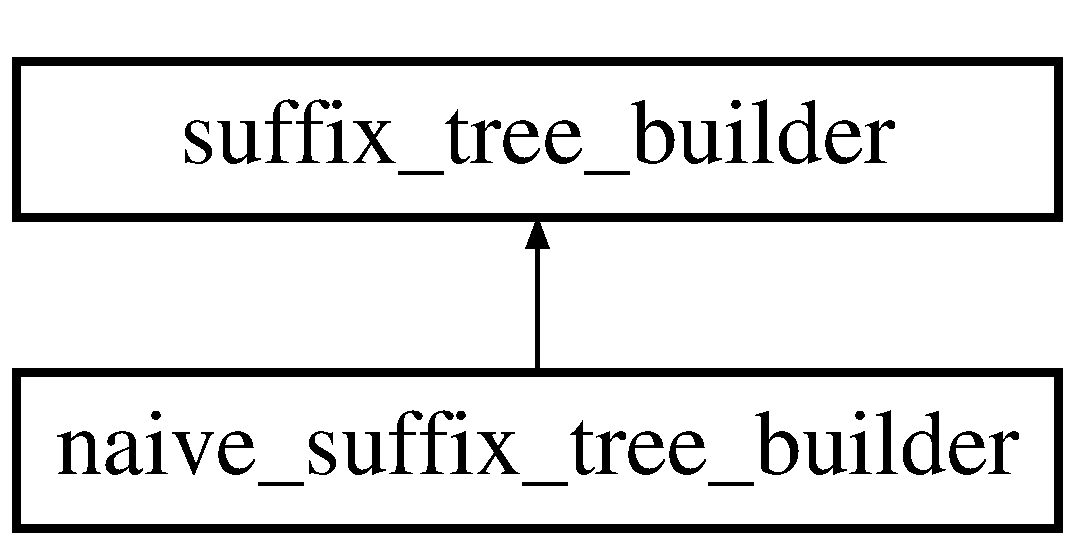
\includegraphics[height=2.000000cm]{classnaive__suffix__tree__builder}
\end{center}
\end{figure}
\subsection*{Public Member Functions}
\begin{DoxyCompactItemize}
\item 
\hypertarget{classnaive__suffix__tree__builder_a4f6133321fe57fc7fe25b08df26f43fd}{\hyperlink{classsuffix__tree}{suffix\+\_\+tree} $\ast$ {\bfseries build\+\_\+tree} (const string \&haystack)}\label{classnaive__suffix__tree__builder_a4f6133321fe57fc7fe25b08df26f43fd}

\item 
\hypertarget{classnaive__suffix__tree__builder_ab7accd6a62ec6e9469e3e8080d270b2f}{\hyperlink{classsuffix__tree}{suffix\+\_\+tree} $\ast$ {\bfseries build\+\_\+tree} (const char $\ast$haystack, int length=-\/1)}\label{classnaive__suffix__tree__builder_ab7accd6a62ec6e9469e3e8080d270b2f}

\item 
\hypertarget{classnaive__suffix__tree__builder_a0d87a4f6d8c106f0db372fd7cc7c9a16}{void {\bfseries branch} (int index, int start\+\_\+s, int end\+\_\+s, \hyperlink{classsuffix__tree_1_1node}{suffix\+\_\+tree\+::node} $\ast$from, \hyperlink{classsuffix__tree_1_1node}{suffix\+\_\+tree\+::node} $\ast$to, \hyperlink{classsuffix__tree_1_1edge}{suffix\+\_\+tree\+::edge} $\ast$e)}\label{classnaive__suffix__tree__builder_a0d87a4f6d8c106f0db372fd7cc7c9a16}

\end{DoxyCompactItemize}
\subsection*{Additional Inherited Members}


The documentation for this class was generated from the following file\+:\begin{DoxyCompactItemize}
\item 
structures/naive\+\_\+suffix\+\_\+tree\+\_\+builder.\+hpp\end{DoxyCompactItemize}

\hypertarget{classsuffix__trie_1_1node}{\section{suffix\+\_\+trie\+:\+:node Class Reference}
\label{classsuffix__trie_1_1node}\index{suffix\+\_\+trie\+::node@{suffix\+\_\+trie\+::node}}
}


{\ttfamily \#include $<$suffix\+\_\+trie.\+hpp$>$}

\subsection*{Public Member Functions}
\begin{DoxyCompactItemize}
\item 
bool \hyperlink{classsuffix__trie_1_1node_a480aaa8ea25e04ac11a8dd470a957265}{edge\+\_\+exists} (char index)
\item 
\hyperlink{classsuffix__trie_1_1edge}{suffix\+\_\+trie\+::edge} $\ast$ \hyperlink{classsuffix__trie_1_1node_ac4e1886521e0e4140aae9556bdaa5631}{get\+\_\+edge} (char index)
\item 
void \hyperlink{classsuffix__trie_1_1node_adfb2fe365b990b61a1b91db8f5d3749a}{add\+\_\+edge} (char index, \hyperlink{classsuffix__trie_1_1edge}{suffix\+\_\+trie\+::edge} $\ast$e)
\item 
map$<$ char, \hyperlink{classsuffix__trie_1_1edge}{suffix\+\_\+trie\+::edge} $\ast$ $>$ \hyperlink{classsuffix__trie_1_1node_a740a3d23a9fe2b31e3066393b22ed099}{get\+\_\+edges} ()
\item 
\hyperlink{classsuffix__trie_1_1node_a495615a4cd50f64bc2455d7a8e8d9cbe}{$\sim$node} ()
\end{DoxyCompactItemize}
\subsection*{Friends}
\begin{DoxyCompactItemize}
\item 
ostream \& \hyperlink{classsuffix__trie_1_1node_ac4586c42ed86200a853773383056f379}{operator$<$$<$} (ostream \&stream, \hyperlink{classsuffix__trie_1_1node}{node} \&c\+\_\+node)
\end{DoxyCompactItemize}


\subsection{Detailed Description}
{\itshape node} is the node in the tree 

\subsection{Constructor \& Destructor Documentation}
\hypertarget{classsuffix__trie_1_1node_a495615a4cd50f64bc2455d7a8e8d9cbe}{\index{suffix\+\_\+trie\+::node@{suffix\+\_\+trie\+::node}!````~node@{$\sim$node}}
\index{````~node@{$\sim$node}!suffix\+\_\+trie\+::node@{suffix\+\_\+trie\+::node}}
\subsubsection[{$\sim$node}]{\setlength{\rightskip}{0pt plus 5cm}suffix\+\_\+trie\+::node\+::$\sim$node (
\begin{DoxyParamCaption}
{}
\end{DoxyParamCaption}
)}}\label{classsuffix__trie_1_1node_a495615a4cd50f64bc2455d7a8e8d9cbe}
destroys the node. It will also destroy recursively all edges and nodes. 

\subsection{Member Function Documentation}
\hypertarget{classsuffix__trie_1_1node_adfb2fe365b990b61a1b91db8f5d3749a}{\index{suffix\+\_\+trie\+::node@{suffix\+\_\+trie\+::node}!add\+\_\+edge@{add\+\_\+edge}}
\index{add\+\_\+edge@{add\+\_\+edge}!suffix\+\_\+trie\+::node@{suffix\+\_\+trie\+::node}}
\subsubsection[{add\+\_\+edge}]{\setlength{\rightskip}{0pt plus 5cm}void suffix\+\_\+trie\+::node\+::add\+\_\+edge (
\begin{DoxyParamCaption}
\item[{char}]{index, }
\item[{{\bf suffix\+\_\+trie\+::edge} $\ast$}]{e}
\end{DoxyParamCaption}
)}}\label{classsuffix__trie_1_1node_adfb2fe365b990b61a1b91db8f5d3749a}
adds an {\itshape edge} {\itshape e} with a given index. \hypertarget{classsuffix__trie_1_1node_a480aaa8ea25e04ac11a8dd470a957265}{\index{suffix\+\_\+trie\+::node@{suffix\+\_\+trie\+::node}!edge\+\_\+exists@{edge\+\_\+exists}}
\index{edge\+\_\+exists@{edge\+\_\+exists}!suffix\+\_\+trie\+::node@{suffix\+\_\+trie\+::node}}
\subsubsection[{edge\+\_\+exists}]{\setlength{\rightskip}{0pt plus 5cm}bool suffix\+\_\+trie\+::node\+::edge\+\_\+exists (
\begin{DoxyParamCaption}
\item[{char}]{index}
\end{DoxyParamCaption}
)}}\label{classsuffix__trie_1_1node_a480aaa8ea25e04ac11a8dd470a957265}
return true if the edge is stored in the map. \hypertarget{classsuffix__trie_1_1node_ac4e1886521e0e4140aae9556bdaa5631}{\index{suffix\+\_\+trie\+::node@{suffix\+\_\+trie\+::node}!get\+\_\+edge@{get\+\_\+edge}}
\index{get\+\_\+edge@{get\+\_\+edge}!suffix\+\_\+trie\+::node@{suffix\+\_\+trie\+::node}}
\subsubsection[{get\+\_\+edge}]{\setlength{\rightskip}{0pt plus 5cm}{\bf suffix\+\_\+trie\+::edge} $\ast$ suffix\+\_\+trie\+::node\+::get\+\_\+edge (
\begin{DoxyParamCaption}
\item[{char}]{index}
\end{DoxyParamCaption}
)}}\label{classsuffix__trie_1_1node_ac4e1886521e0e4140aae9556bdaa5631}
return a pointer to a {\itshape \hyperlink{classsuffix__trie_1_1edge}{suffix\+\_\+trie\+::edge}} with a given index(key) \hypertarget{classsuffix__trie_1_1node_a740a3d23a9fe2b31e3066393b22ed099}{\index{suffix\+\_\+trie\+::node@{suffix\+\_\+trie\+::node}!get\+\_\+edges@{get\+\_\+edges}}
\index{get\+\_\+edges@{get\+\_\+edges}!suffix\+\_\+trie\+::node@{suffix\+\_\+trie\+::node}}
\subsubsection[{get\+\_\+edges}]{\setlength{\rightskip}{0pt plus 5cm}map$<$ char, {\bf suffix\+\_\+trie\+::edge} $\ast$ $>$ suffix\+\_\+trie\+::node\+::get\+\_\+edges (
\begin{DoxyParamCaption}
{}
\end{DoxyParamCaption}
)}}\label{classsuffix__trie_1_1node_a740a3d23a9fe2b31e3066393b22ed099}
returns all outgoing edges 

\subsection{Friends And Related Function Documentation}
\hypertarget{classsuffix__trie_1_1node_ac4586c42ed86200a853773383056f379}{\index{suffix\+\_\+trie\+::node@{suffix\+\_\+trie\+::node}!operator$<$$<$@{operator$<$$<$}}
\index{operator$<$$<$@{operator$<$$<$}!suffix\+\_\+trie\+::node@{suffix\+\_\+trie\+::node}}
\subsubsection[{operator$<$$<$}]{\setlength{\rightskip}{0pt plus 5cm}ostream\& operator$<$$<$ (
\begin{DoxyParamCaption}
\item[{ostream \&}]{stream, }
\item[{{\bf suffix\+\_\+trie\+::node} \&}]{c\+\_\+node}
\end{DoxyParamCaption}
)\hspace{0.3cm}{\ttfamily [friend]}}}\label{classsuffix__trie_1_1node_ac4586c42ed86200a853773383056f379}
overrides the $<$$<$ operator for printing the node 

The documentation for this class was generated from the following files\+:\begin{DoxyCompactItemize}
\item 
structures/\hyperlink{suffix__trie_8hpp}{suffix\+\_\+trie.\+hpp}\item 
structures/suffix\+\_\+trie.\+cpp\end{DoxyCompactItemize}

\hypertarget{classsuffix__tree_1_1node}{\section{suffix\+\_\+tree\+:\+:node Class Reference}
\label{classsuffix__tree_1_1node}\index{suffix\+\_\+tree\+::node@{suffix\+\_\+tree\+::node}}
}
\subsection*{Public Member Functions}
\begin{DoxyCompactItemize}
\item 
\hypertarget{classsuffix__tree_1_1node_a7a6ccca904c47d555e55e4aba1ebd99c}{{\bfseries node} (int index)}\label{classsuffix__tree_1_1node_a7a6ccca904c47d555e55e4aba1ebd99c}

\item 
\hypertarget{classsuffix__tree_1_1node_abb452bc081d5f178819e5987c3fb6bbc}{int {\bfseries get\+\_\+index} ()}\label{classsuffix__tree_1_1node_abb452bc081d5f178819e5987c3fb6bbc}

\item 
\hypertarget{classsuffix__tree_1_1node_ad0d7685baec672218057823831903b78}{void {\bfseries add\+\_\+edge} (\hyperlink{classsuffix__tree_1_1edge}{edge} $\ast$e, char index)}\label{classsuffix__tree_1_1node_ad0d7685baec672218057823831903b78}

\item 
\hypertarget{classsuffix__tree_1_1node_ac0a751778ca1452fbb03c22624d27169}{\hyperlink{classsuffix__tree_1_1edge}{edge} $\ast$ {\bfseries get\+\_\+edge} (char index)}\label{classsuffix__tree_1_1node_ac0a751778ca1452fbb03c22624d27169}

\item 
\hypertarget{classsuffix__tree_1_1node_a9f5e36d0541512b1f3de7c5de889bfe1}{bool {\bfseries has\+\_\+edge} (char index)}\label{classsuffix__tree_1_1node_a9f5e36d0541512b1f3de7c5de889bfe1}

\end{DoxyCompactItemize}


The documentation for this class was generated from the following files\+:\begin{DoxyCompactItemize}
\item 
structures/suffix\+\_\+tree.\+hpp\item 
structures/suffix\+\_\+tree.\+cpp\end{DoxyCompactItemize}

\hypertarget{classrabin__karp__searcher}{\section{rabin\+\_\+karp\+\_\+searcher Class Reference}
\label{classrabin__karp__searcher}\index{rabin\+\_\+karp\+\_\+searcher@{rabin\+\_\+karp\+\_\+searcher}}
}
\subsection*{Public Member Functions}
\begin{DoxyCompactItemize}
\item 
\hypertarget{classrabin__karp__searcher_af87b49667bfaae8aa9e04c40a56ef65d}{void {\bfseries compute\+\_\+powers} (int power)}\label{classrabin__karp__searcher_af87b49667bfaae8aa9e04c40a56ef65d}

\item 
\hypertarget{classrabin__karp__searcher_a8e84f35d889d207d2e1d8f1667b096f1}{int {\bfseries rabin\+\_\+karp\+\_\+search} (const string \&haystack, const string \&needle, int start=0)}\label{classrabin__karp__searcher_a8e84f35d889d207d2e1d8f1667b096f1}

\item 
\hypertarget{classrabin__karp__searcher_a463e7806633823f5e0b337d5751c0941}{int {\bfseries rabin\+\_\+karp\+\_\+search} (const char $\ast$haystack, const char $\ast$needle, int start=0, int haystack\+\_\+length=-\/1, int needle\+\_\+length=-\/1)}\label{classrabin__karp__searcher_a463e7806633823f5e0b337d5751c0941}

\item 
\hypertarget{classrabin__karp__searcher_abfdd295c35e50777268b2c93c0d63cf1}{bool {\bfseries check\+\_\+equals} (const char $\ast$haystack, const char $\ast$needle, int index, int needle\+\_\+length)}\label{classrabin__karp__searcher_abfdd295c35e50777268b2c93c0d63cf1}

\end{DoxyCompactItemize}


The documentation for this class was generated from the following files\+:\begin{DoxyCompactItemize}
\item 
algorithms/rabin\+\_\+karp.\+hpp\item 
algorithms/rabin\+\_\+karp.\+cpp\end{DoxyCompactItemize}

\hypertarget{classsuffix__tree}{\section{suffix\+\_\+tree Class Reference}
\label{classsuffix__tree}\index{suffix\+\_\+tree@{suffix\+\_\+tree}}
}
\subsection*{Classes}
\begin{DoxyCompactItemize}
\item 
class \hyperlink{classsuffix__tree_1_1edge}{edge}
\item 
class \hyperlink{classsuffix__tree_1_1node}{node}
\end{DoxyCompactItemize}
\subsection*{Public Member Functions}
\begin{DoxyCompactItemize}
\item 
\hypertarget{classsuffix__tree_acbe8b85bf66af768b42622f58e403c99}{{\bfseries suffix\+\_\+tree} (\hyperlink{classsuffix__tree_1_1node}{node} $\ast$root)}\label{classsuffix__tree_acbe8b85bf66af768b42622f58e403c99}

\item 
\hypertarget{classsuffix__tree_ad196450a7bf1ef5cbaf853093555194f}{int {\bfseries get\+\_\+first\+\_\+occurrence} (const string \&needle)}\label{classsuffix__tree_ad196450a7bf1ef5cbaf853093555194f}

\item 
\hypertarget{classsuffix__tree_aef9a13a219454fbc05eef02c92ad4a33}{int {\bfseries get\+\_\+first\+\_\+occurrence} (const char $\ast$needle, int length=-\/1)}\label{classsuffix__tree_aef9a13a219454fbc05eef02c92ad4a33}

\item 
\hypertarget{classsuffix__tree_a679b725baeb7ca34d9e5e87653ed452e}{vector$<$ int $>$ {\bfseries get\+\_\+all\+\_\+occurrences} (const string \&needle)}\label{classsuffix__tree_a679b725baeb7ca34d9e5e87653ed452e}

\item 
\hypertarget{classsuffix__tree_a82bf896df6938cefbe2a097b685f8821}{vector$<$ int $>$ {\bfseries get\+\_\+all\+\_\+occurrences} (const char $\ast$needle, int length=-\/1)}\label{classsuffix__tree_a82bf896df6938cefbe2a097b685f8821}

\end{DoxyCompactItemize}


The documentation for this class was generated from the following file\+:\begin{DoxyCompactItemize}
\item 
structures/suffix\+\_\+tree.\+hpp\end{DoxyCompactItemize}

\hypertarget{classsuffix__tree__builder}{\section{suffix\+\_\+tree\+\_\+builder Class Reference}
\label{classsuffix__tree__builder}\index{suffix\+\_\+tree\+\_\+builder@{suffix\+\_\+tree\+\_\+builder}}
}
Inheritance diagram for suffix\+\_\+tree\+\_\+builder\+:\begin{figure}[H]
\begin{center}
\leavevmode
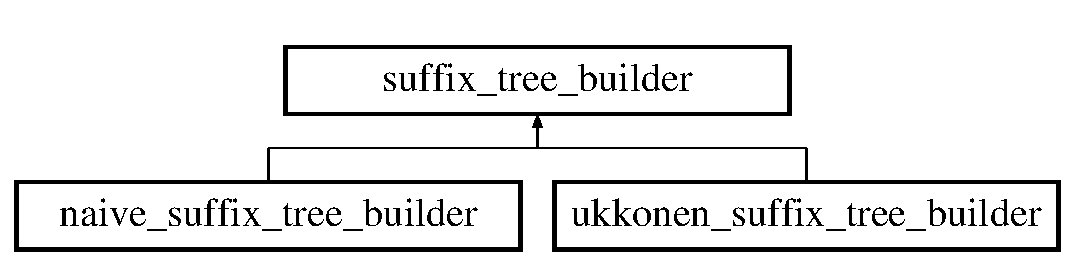
\includegraphics[height=2.000000cm]{classsuffix__tree__builder}
\end{center}
\end{figure}
\subsection*{Public Member Functions}
\begin{DoxyCompactItemize}
\item 
\hypertarget{classsuffix__tree__builder_aff50e4acf552359f8c72130b9c589825}{virtual \hyperlink{classsuffix__tree}{suffix\+\_\+tree} $\ast$ {\bfseries build\+\_\+tree} (const string \&haystack)=0}\label{classsuffix__tree__builder_aff50e4acf552359f8c72130b9c589825}

\item 
\hypertarget{classsuffix__tree__builder_a1dd1414a13def280ee9f1b90a46d6371}{virtual \hyperlink{classsuffix__tree}{suffix\+\_\+tree} $\ast$ {\bfseries build\+\_\+tree} (const char $\ast$haystack, int length=-\/1)=0}\label{classsuffix__tree__builder_a1dd1414a13def280ee9f1b90a46d6371}

\end{DoxyCompactItemize}
\subsection*{Static Protected Attributes}
\begin{DoxyCompactItemize}
\item 
\hypertarget{classsuffix__tree__builder_a50d71959120fb1a65cae59b7288d7dd4}{static const char {\bfseries stop\+\_\+char} = '\textbackslash{}0'}\label{classsuffix__tree__builder_a50d71959120fb1a65cae59b7288d7dd4}

\end{DoxyCompactItemize}


The documentation for this class was generated from the following file\+:\begin{DoxyCompactItemize}
\item 
structures/suffix\+\_\+tree\+\_\+builder.\+hpp\end{DoxyCompactItemize}

\hypertarget{classsuffix__trie}{\section{suffix\+\_\+trie Class Reference}
\label{classsuffix__trie}\index{suffix\+\_\+trie@{suffix\+\_\+trie}}
}


{\ttfamily \#include $<$suffix\+\_\+trie.\+hpp$>$}

\subsection*{Classes}
\begin{DoxyCompactItemize}
\item 
class \hyperlink{classsuffix__trie_1_1edge}{edge}
\item 
class \hyperlink{classsuffix__trie_1_1node}{node}
\end{DoxyCompactItemize}
\subsection*{Public Member Functions}
\begin{DoxyCompactItemize}
\item 
\hyperlink{classsuffix__trie_a9abcb4670f7a77310cb99b9bcf793d96}{suffix\+\_\+trie} (\hyperlink{classsuffix__trie_1_1node}{node} $\ast$root)
\item 
\hyperlink{classsuffix__trie_ad167499438414cfd39d4348293ce518c}{$\sim$suffix\+\_\+trie} ()
\item 
int \hyperlink{classsuffix__trie_aa0b4eb1f5b48c368bab4e7fa092f3397}{find\+\_\+first} (const char $\ast$needle, int needle\+\_\+length=-\/1)
\item 
int \hyperlink{classsuffix__trie_ace4532672b5494b16ca6a61ece4253bb}{find\+\_\+first} (const string \&needle)
\item 
vector$<$ int $>$ \hyperlink{classsuffix__trie_ab362340e269e59692d4fabe133d15a6c}{find\+\_\+all} (const char $\ast$needle, int needle\+\_\+length=-\/1)
\item 
vector$<$ int $>$ \hyperlink{classsuffix__trie_a389b5a98d9de10c0ff9fbd2e2ae7b117}{find\+\_\+all} (const string \&needle)
\item 
\hyperlink{classsuffix__trie_1_1node}{suffix\+\_\+trie\+::node} $\ast$ \hyperlink{classsuffix__trie_aaac718aa91f18353d139d1af068e132b}{get\+\_\+root} ()
\end{DoxyCompactItemize}
\subsection*{Static Public Attributes}
\begin{DoxyCompactItemize}
\item 
static const char \hyperlink{classsuffix__trie_a65563ea1279d3fc3353a0806f6a07aad}{S\+T\+O\+P\+\_\+\+C\+H\+A\+R} = 127
\end{DoxyCompactItemize}
\subsection*{Friends}
\begin{DoxyCompactItemize}
\item 
ostream \& \hyperlink{classsuffix__trie_a01feaa688d57e9a27960b68e168d98ea}{operator$<$$<$} (ostream \&stream, \hyperlink{classsuffix__trie}{suffix\+\_\+trie} \&trie)
\end{DoxyCompactItemize}


\subsection{Detailed Description}
{\itshape \hyperlink{classsuffix__trie}{suffix\+\_\+trie}} is a tree structure which contains information about a given text. It supports searching in the text. 

\subsection{Constructor \& Destructor Documentation}
\hypertarget{classsuffix__trie_a9abcb4670f7a77310cb99b9bcf793d96}{\index{suffix\+\_\+trie@{suffix\+\_\+trie}!suffix\+\_\+trie@{suffix\+\_\+trie}}
\index{suffix\+\_\+trie@{suffix\+\_\+trie}!suffix\+\_\+trie@{suffix\+\_\+trie}}
\subsubsection[{suffix\+\_\+trie}]{\setlength{\rightskip}{0pt plus 5cm}suffix\+\_\+trie\+::suffix\+\_\+trie (
\begin{DoxyParamCaption}
\item[{{\bf node} $\ast$}]{root}
\end{DoxyParamCaption}
)}}\label{classsuffix__trie_a9abcb4670f7a77310cb99b9bcf793d96}
creates a {\itshape \hyperlink{classsuffix__trie}{suffix\+\_\+trie}} with a given {\itshape \hyperlink{classsuffix__trie_1_1node}{suffix\+\_\+trie\+::node}} root pointer \hypertarget{classsuffix__trie_ad167499438414cfd39d4348293ce518c}{\index{suffix\+\_\+trie@{suffix\+\_\+trie}!````~suffix\+\_\+trie@{$\sim$suffix\+\_\+trie}}
\index{````~suffix\+\_\+trie@{$\sim$suffix\+\_\+trie}!suffix\+\_\+trie@{suffix\+\_\+trie}}
\subsubsection[{$\sim$suffix\+\_\+trie}]{\setlength{\rightskip}{0pt plus 5cm}suffix\+\_\+trie\+::$\sim$suffix\+\_\+trie (
\begin{DoxyParamCaption}
{}
\end{DoxyParamCaption}
)}}\label{classsuffix__trie_ad167499438414cfd39d4348293ce518c}
destroys the suffix trie and all of its nodes and edges recursively 

\subsection{Member Function Documentation}
\hypertarget{classsuffix__trie_ab362340e269e59692d4fabe133d15a6c}{\index{suffix\+\_\+trie@{suffix\+\_\+trie}!find\+\_\+all@{find\+\_\+all}}
\index{find\+\_\+all@{find\+\_\+all}!suffix\+\_\+trie@{suffix\+\_\+trie}}
\subsubsection[{find\+\_\+all}]{\setlength{\rightskip}{0pt plus 5cm}vector$<$int$>$ suffix\+\_\+trie\+::find\+\_\+all (
\begin{DoxyParamCaption}
\item[{const char $\ast$}]{needle, }
\item[{int}]{needle\+\_\+length = {\ttfamily -\/1}}
\end{DoxyParamCaption}
)}}\label{classsuffix__trie_ab362340e269e59692d4fabe133d15a6c}
returns all occurrences of the {\itshape needle} in the preprocessed text. If {\itshape needle\+\_\+length} is ommited, then the length is computed by using strlen(). \hypertarget{classsuffix__trie_a389b5a98d9de10c0ff9fbd2e2ae7b117}{\index{suffix\+\_\+trie@{suffix\+\_\+trie}!find\+\_\+all@{find\+\_\+all}}
\index{find\+\_\+all@{find\+\_\+all}!suffix\+\_\+trie@{suffix\+\_\+trie}}
\subsubsection[{find\+\_\+all}]{\setlength{\rightskip}{0pt plus 5cm}vector$<$int$>$ suffix\+\_\+trie\+::find\+\_\+all (
\begin{DoxyParamCaption}
\item[{const string \&}]{needle}
\end{DoxyParamCaption}
)}}\label{classsuffix__trie_a389b5a98d9de10c0ff9fbd2e2ae7b117}
returns all occurrences of the {\itshape needle} in the preprocessed text. \hypertarget{classsuffix__trie_aa0b4eb1f5b48c368bab4e7fa092f3397}{\index{suffix\+\_\+trie@{suffix\+\_\+trie}!find\+\_\+first@{find\+\_\+first}}
\index{find\+\_\+first@{find\+\_\+first}!suffix\+\_\+trie@{suffix\+\_\+trie}}
\subsubsection[{find\+\_\+first}]{\setlength{\rightskip}{0pt plus 5cm}int suffix\+\_\+trie\+::find\+\_\+first (
\begin{DoxyParamCaption}
\item[{const char $\ast$}]{needle, }
\item[{int}]{needle\+\_\+length = {\ttfamily -\/1}}
\end{DoxyParamCaption}
)}}\label{classsuffix__trie_aa0b4eb1f5b48c368bab4e7fa092f3397}
returns the first occurrence of the {\itshape needle} in the preprocessed text. If {\itshape needle\+\_\+length} is ommited, then the length is computed by using strlen(). \hypertarget{classsuffix__trie_ace4532672b5494b16ca6a61ece4253bb}{\index{suffix\+\_\+trie@{suffix\+\_\+trie}!find\+\_\+first@{find\+\_\+first}}
\index{find\+\_\+first@{find\+\_\+first}!suffix\+\_\+trie@{suffix\+\_\+trie}}
\subsubsection[{find\+\_\+first}]{\setlength{\rightskip}{0pt plus 5cm}int suffix\+\_\+trie\+::find\+\_\+first (
\begin{DoxyParamCaption}
\item[{const string \&}]{needle}
\end{DoxyParamCaption}
)}}\label{classsuffix__trie_ace4532672b5494b16ca6a61ece4253bb}
returns the first occurrence of the {\itshape needle} in the preprocessed text. \hypertarget{classsuffix__trie_aaac718aa91f18353d139d1af068e132b}{\index{suffix\+\_\+trie@{suffix\+\_\+trie}!get\+\_\+root@{get\+\_\+root}}
\index{get\+\_\+root@{get\+\_\+root}!suffix\+\_\+trie@{suffix\+\_\+trie}}
\subsubsection[{get\+\_\+root}]{\setlength{\rightskip}{0pt plus 5cm}{\bf suffix\+\_\+trie\+::node} $\ast$ suffix\+\_\+trie\+::get\+\_\+root (
\begin{DoxyParamCaption}
{}
\end{DoxyParamCaption}
)}}\label{classsuffix__trie_aaac718aa91f18353d139d1af068e132b}
returns the root of the trie 

\subsection{Friends And Related Function Documentation}
\hypertarget{classsuffix__trie_a01feaa688d57e9a27960b68e168d98ea}{\index{suffix\+\_\+trie@{suffix\+\_\+trie}!operator$<$$<$@{operator$<$$<$}}
\index{operator$<$$<$@{operator$<$$<$}!suffix\+\_\+trie@{suffix\+\_\+trie}}
\subsubsection[{operator$<$$<$}]{\setlength{\rightskip}{0pt plus 5cm}ostream\& operator$<$$<$ (
\begin{DoxyParamCaption}
\item[{ostream \&}]{stream, }
\item[{{\bf suffix\+\_\+trie} \&}]{trie}
\end{DoxyParamCaption}
)\hspace{0.3cm}{\ttfamily [friend]}}}\label{classsuffix__trie_a01feaa688d57e9a27960b68e168d98ea}
overrides the $<$$<$ operator to print the {\itshape \hyperlink{classsuffix__trie}{suffix\+\_\+trie}} 

\subsection{Member Data Documentation}
\hypertarget{classsuffix__trie_a65563ea1279d3fc3353a0806f6a07aad}{\index{suffix\+\_\+trie@{suffix\+\_\+trie}!S\+T\+O\+P\+\_\+\+C\+H\+A\+R@{S\+T\+O\+P\+\_\+\+C\+H\+A\+R}}
\index{S\+T\+O\+P\+\_\+\+C\+H\+A\+R@{S\+T\+O\+P\+\_\+\+C\+H\+A\+R}!suffix\+\_\+trie@{suffix\+\_\+trie}}
\subsubsection[{S\+T\+O\+P\+\_\+\+C\+H\+A\+R}]{\setlength{\rightskip}{0pt plus 5cm}const char suffix\+\_\+trie\+::\+S\+T\+O\+P\+\_\+\+C\+H\+A\+R = 127\hspace{0.3cm}{\ttfamily [static]}}}\label{classsuffix__trie_a65563ea1279d3fc3353a0806f6a07aad}
stop character which is added to the end of the string 

The documentation for this class was generated from the following files\+:\begin{DoxyCompactItemize}
\item 
structures/\hyperlink{suffix__trie_8hpp}{suffix\+\_\+trie.\+hpp}\item 
structures/suffix\+\_\+trie.\+cpp\end{DoxyCompactItemize}

\hypertarget{classsuffix__trie__builder}{\section{suffix\+\_\+trie\+\_\+builder Class Reference}
\label{classsuffix__trie__builder}\index{suffix\+\_\+trie\+\_\+builder@{suffix\+\_\+trie\+\_\+builder}}
}


{\ttfamily \#include $<$suffix\+\_\+trie\+\_\+builder.\+hpp$>$}



\subsection{Detailed Description}
{\itshape \hyperlink{classsuffix__trie__builder}{suffix\+\_\+trie\+\_\+builder}} has the purpose to build a suffix trie from a given string 

The documentation for this class was generated from the following files\+:\begin{DoxyCompactItemize}
\item 
structures/\hyperlink{suffix__trie__builder_8hpp}{suffix\+\_\+trie\+\_\+builder.\+hpp}\item 
structures/suffix\+\_\+trie\+\_\+builder.\+cpp\end{DoxyCompactItemize}

\hypertarget{classukkonen__suffix__tree__builder}{\section{ukkonen\+\_\+suffix\+\_\+tree\+\_\+builder Class Reference}
\label{classukkonen__suffix__tree__builder}\index{ukkonen\+\_\+suffix\+\_\+tree\+\_\+builder@{ukkonen\+\_\+suffix\+\_\+tree\+\_\+builder}}
}
Inheritance diagram for ukkonen\+\_\+suffix\+\_\+tree\+\_\+builder\+:\begin{figure}[H]
\begin{center}
\leavevmode
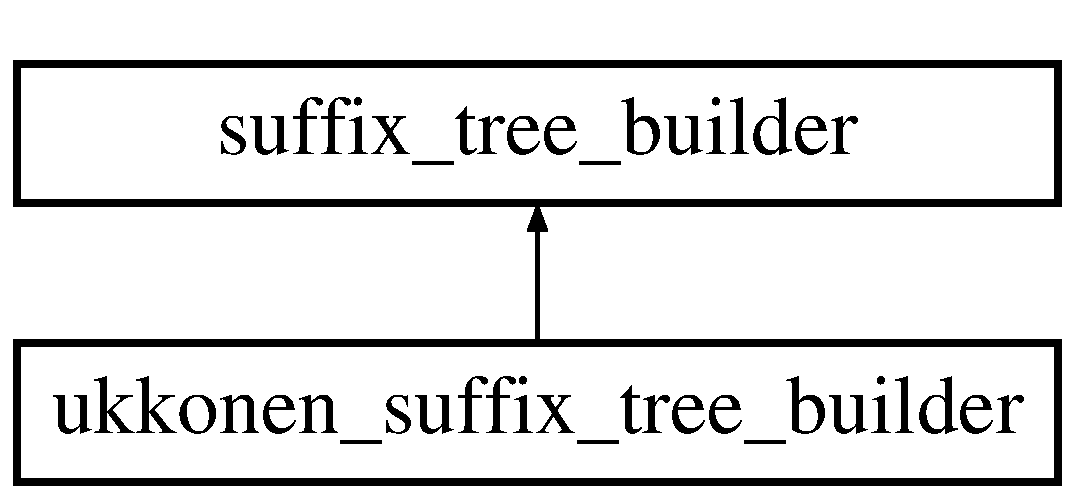
\includegraphics[height=2.000000cm]{classukkonen__suffix__tree__builder}
\end{center}
\end{figure}
\subsection*{Additional Inherited Members}


The documentation for this class was generated from the following file\+:\begin{DoxyCompactItemize}
\item 
structures/ukkonen\+\_\+suffix\+\_\+tree\+\_\+builder.\+hpp\end{DoxyCompactItemize}

\chapter{File Documentation}
\hypertarget{edit__distance_8hpp}{\section{algorithms/edit\+\_\+distance.hpp File Reference}
\label{edit__distance_8hpp}\index{algorithms/edit\+\_\+distance.\+hpp@{algorithms/edit\+\_\+distance.\+hpp}}
}
{\ttfamily \#include $<$cstring$>$}\\*
{\ttfamily \#include $<$string$>$}\\*
{\ttfamily \#include $<$cstdlib$>$}\\*
\subsection*{Classes}
\begin{DoxyCompactItemize}
\item 
class \hyperlink{classedit__distance}{edit\+\_\+distance}
\end{DoxyCompactItemize}

\hypertarget{naive_8hpp}{\section{algorithms/naive.hpp File Reference}
\label{naive_8hpp}\index{algorithms/naive.\+hpp@{algorithms/naive.\+hpp}}
}
{\ttfamily \#include \char`\"{}../constants.\+hpp\char`\"{}}\\*
{\ttfamily \#include $<$cstring$>$}\\*
{\ttfamily \#include $<$string$>$}\\*
\subsection*{Functions}
\begin{DoxyCompactItemize}
\item 
int \hyperlink{naive_8hpp_a7df3168ae10755c311800c8b2a88385d}{naive\+\_\+search} (const string \&haystack, const string \&needle, int start=0)
\item 
int \hyperlink{naive_8hpp_a88a31f9a8cc8b9a8b2d83b0bc6cedb54}{naive\+\_\+search} (const char $\ast$haystack, const char $\ast$needle, int start=0, int haystack\+\_\+length=-\/1, int needle\+\_\+length=-\/1)
\end{DoxyCompactItemize}


\subsection{Function Documentation}
\hypertarget{naive_8hpp_a7df3168ae10755c311800c8b2a88385d}{\index{naive.\+hpp@{naive.\+hpp}!naive\+\_\+search@{naive\+\_\+search}}
\index{naive\+\_\+search@{naive\+\_\+search}!naive.\+hpp@{naive.\+hpp}}
\subsubsection[{naive\+\_\+search}]{\setlength{\rightskip}{0pt plus 5cm}int naive\+\_\+search (
\begin{DoxyParamCaption}
\item[{const string \&}]{haystack, }
\item[{const string \&}]{needle, }
\item[{int}]{start = {\ttfamily 0}}
\end{DoxyParamCaption}
)}}\label{naive_8hpp_a7df3168ae10755c311800c8b2a88385d}
returns a found index of {\itshape needle} in {\itshape haystack} after an index {\itshape start}. By default {\itshape start} has value 0. \hypertarget{naive_8hpp_a88a31f9a8cc8b9a8b2d83b0bc6cedb54}{\index{naive.\+hpp@{naive.\+hpp}!naive\+\_\+search@{naive\+\_\+search}}
\index{naive\+\_\+search@{naive\+\_\+search}!naive.\+hpp@{naive.\+hpp}}
\subsubsection[{naive\+\_\+search}]{\setlength{\rightskip}{0pt plus 5cm}int naive\+\_\+search (
\begin{DoxyParamCaption}
\item[{const char $\ast$}]{haystack, }
\item[{const char $\ast$}]{needle, }
\item[{int}]{start = {\ttfamily 0}, }
\item[{int}]{haystack\+\_\+length = {\ttfamily -\/1}, }
\item[{int}]{needle\+\_\+length = {\ttfamily -\/1}}
\end{DoxyParamCaption}
)}}\label{naive_8hpp_a88a31f9a8cc8b9a8b2d83b0bc6cedb54}
returns a found index of {\itshape needle} in {\itshape haystack} after an index {\itshape start}, where {\itshape needle} has length {\itshape haystack\+\_\+length} and {\itshape needle} has length {\itshape needle\+\_\+length}. 
\hypertarget{rabin__karp_8hpp}{\section{algorithms/rabin\+\_\+karp.hpp File Reference}
\label{rabin__karp_8hpp}\index{algorithms/rabin\+\_\+karp.\+hpp@{algorithms/rabin\+\_\+karp.\+hpp}}
}
{\ttfamily \#include $<$cstring$>$}\\*
{\ttfamily \#include $<$string$>$}\\*
{\ttfamily \#include $<$iostream$>$}\\*
{\ttfamily \#include $<$cstdlib$>$}\\*
{\ttfamily \#include \char`\"{}../constants.\+hpp\char`\"{}}\\*
\subsection*{Classes}
\begin{DoxyCompactItemize}
\item 
class \hyperlink{classrabin__karp__searcher}{rabin\+\_\+karp\+\_\+searcher}
\end{DoxyCompactItemize}

\hypertarget{z__algorithm_8hpp}{\section{algorithms/z\+\_\+algorithm.hpp File Reference}
\label{z__algorithm_8hpp}\index{algorithms/z\+\_\+algorithm.\+hpp@{algorithms/z\+\_\+algorithm.\+hpp}}
}
{\ttfamily \#include $<$cstring$>$}\\*
{\ttfamily \#include $<$string$>$}\\*
{\ttfamily \#include $<$vector$>$}\\*
{\ttfamily \#include $<$cstdlib$>$}\\*
\subsection*{Functions}
\begin{DoxyCompactItemize}
\item 
bool \hyperlink{z__algorithm_8hpp_af7c7f1543758fd971c84df769efaca2a}{z\+\_\+algo\+\_\+compare} (const char $\ast$haystack, const char $\ast$needle, int index\+\_\+a, int index\+\_\+b, int haystack\+\_\+length, int needle\+\_\+length)
\item 
vector$<$ int $>$ \hyperlink{z__algorithm_8hpp_a6e993244fe95494de6686ee986f36503}{z\+\_\+algo\+\_\+get\+\_\+positions} (const string \&haystack, const string \&needle, int start=0, int upper\+\_\+bound\+\_\+cnt=-\/1)
\item 
vector$<$ int $>$ \hyperlink{z__algorithm_8hpp_ac4a25bd217172483c570b87b5cb9a86b}{z\+\_\+algo\+\_\+get\+\_\+positions} (const char $\ast$haystack, const char $\ast$needle, int start=0, int haystack\+\_\+length=-\/1, int needle\+\_\+length=-\/1, int upper\+\_\+bound\+\_\+cnt=-\/1)
\item 
void \hyperlink{z__algorithm_8hpp_a273289996997b353d250953ac4d288ec}{extend\+\_\+right} (int \&right, int left, int total\+\_\+length, const char $\ast$haystack, const char $\ast$needle, int haystack\+\_\+length, int needle\+\_\+length, int start)
\end{DoxyCompactItemize}


\subsection{Function Documentation}
\hypertarget{z__algorithm_8hpp_a273289996997b353d250953ac4d288ec}{\index{z\+\_\+algorithm.\+hpp@{z\+\_\+algorithm.\+hpp}!extend\+\_\+right@{extend\+\_\+right}}
\index{extend\+\_\+right@{extend\+\_\+right}!z\+\_\+algorithm.\+hpp@{z\+\_\+algorithm.\+hpp}}
\subsubsection[{extend\+\_\+right}]{\setlength{\rightskip}{0pt plus 5cm}void extend\+\_\+right (
\begin{DoxyParamCaption}
\item[{int \&}]{right, }
\item[{int}]{left, }
\item[{int}]{total\+\_\+length, }
\item[{const char $\ast$}]{haystack, }
\item[{const char $\ast$}]{needle, }
\item[{int}]{haystack\+\_\+length, }
\item[{int}]{needle\+\_\+length, }
\item[{int}]{start}
\end{DoxyParamCaption}
)}}\label{z__algorithm_8hpp_a273289996997b353d250953ac4d288ec}
Since the main point of the algorithm is to keep an invariant-\/bound \mbox{[}left;right\mbox{]}, this method extends the bound to the right. Accordingly {\itshape total\+\_\+length} is the length of the z array, {\itshape haystack} is the text we are searching in, {\itshape needle} is the string we are searching for, {\itshape haystack\+\_\+length} is the length of the {\itshape haystack}, {\itshape needle\+\_\+length} is the length of the {\itshape needle}, {\itshape start} is the the offset index we start the search from. The {\itshape start} is needed since the z array is dependent on it. \hypertarget{z__algorithm_8hpp_af7c7f1543758fd971c84df769efaca2a}{\index{z\+\_\+algorithm.\+hpp@{z\+\_\+algorithm.\+hpp}!z\+\_\+algo\+\_\+compare@{z\+\_\+algo\+\_\+compare}}
\index{z\+\_\+algo\+\_\+compare@{z\+\_\+algo\+\_\+compare}!z\+\_\+algorithm.\+hpp@{z\+\_\+algorithm.\+hpp}}
\subsubsection[{z\+\_\+algo\+\_\+compare}]{\setlength{\rightskip}{0pt plus 5cm}bool z\+\_\+algo\+\_\+compare (
\begin{DoxyParamCaption}
\item[{const char $\ast$}]{haystack, }
\item[{const char $\ast$}]{needle, }
\item[{int}]{index\+\_\+a, }
\item[{int}]{index\+\_\+b, }
\item[{int}]{haystack\+\_\+length, }
\item[{int}]{needle\+\_\+length}
\end{DoxyParamCaption}
)}}\label{z__algorithm_8hpp_af7c7f1543758fd971c84df769efaca2a}
Compares the characters in z array at index {\itshape index\+\_\+a} and {\itshape index\+\_\+b}. The z array is not generated, but rather using offset to choose which character in {\itshape haystack} and {\itshape needle} to use. The {\itshape haystack\+\_\+length} and {\itshape the} needle\+\_\+length represent the length of the {\itshape haystack} and the {\itshape needle}. \hypertarget{z__algorithm_8hpp_a6e993244fe95494de6686ee986f36503}{\index{z\+\_\+algorithm.\+hpp@{z\+\_\+algorithm.\+hpp}!z\+\_\+algo\+\_\+get\+\_\+positions@{z\+\_\+algo\+\_\+get\+\_\+positions}}
\index{z\+\_\+algo\+\_\+get\+\_\+positions@{z\+\_\+algo\+\_\+get\+\_\+positions}!z\+\_\+algorithm.\+hpp@{z\+\_\+algorithm.\+hpp}}
\subsubsection[{z\+\_\+algo\+\_\+get\+\_\+positions}]{\setlength{\rightskip}{0pt plus 5cm}vector$<$int$>$ z\+\_\+algo\+\_\+get\+\_\+positions (
\begin{DoxyParamCaption}
\item[{const string \&}]{haystack, }
\item[{const string \&}]{needle, }
\item[{int}]{start = {\ttfamily 0}, }
\item[{int}]{upper\+\_\+bound\+\_\+cnt = {\ttfamily -\/1}}
\end{DoxyParamCaption}
)}}\label{z__algorithm_8hpp_a6e993244fe95494de6686ee986f36503}
The function returns the found positions of the string {\itshape needle} in {\itshape haystack}, starting with an offset {\itshape start} (by default 0) and counting at most {\itshape upper\+\_\+bound\+\_\+cnt} (default -\/1) positions. If {\itshape upper\+\_\+bound\+\_\+cnt} is smaller than 0, then it will find all positions of the {\itshape needle}. \hypertarget{z__algorithm_8hpp_ac4a25bd217172483c570b87b5cb9a86b}{\index{z\+\_\+algorithm.\+hpp@{z\+\_\+algorithm.\+hpp}!z\+\_\+algo\+\_\+get\+\_\+positions@{z\+\_\+algo\+\_\+get\+\_\+positions}}
\index{z\+\_\+algo\+\_\+get\+\_\+positions@{z\+\_\+algo\+\_\+get\+\_\+positions}!z\+\_\+algorithm.\+hpp@{z\+\_\+algorithm.\+hpp}}
\subsubsection[{z\+\_\+algo\+\_\+get\+\_\+positions}]{\setlength{\rightskip}{0pt plus 5cm}vector$<$int$>$ z\+\_\+algo\+\_\+get\+\_\+positions (
\begin{DoxyParamCaption}
\item[{const char $\ast$}]{haystack, }
\item[{const char $\ast$}]{needle, }
\item[{int}]{start = {\ttfamily 0}, }
\item[{int}]{haystack\+\_\+length = {\ttfamily -\/1}, }
\item[{int}]{needle\+\_\+length = {\ttfamily -\/1}, }
\item[{int}]{upper\+\_\+bound\+\_\+cnt = {\ttfamily -\/1}}
\end{DoxyParamCaption}
)}}\label{z__algorithm_8hpp_ac4a25bd217172483c570b87b5cb9a86b}
The function returns the found positions of the string {\itshape needle} in {\itshape haystack}, starting with an offset {\itshape start} (by default 0) and counting at most {\itshape upper\+\_\+bound\+\_\+cnt} (default -\/1) positions. If {\itshape upper\+\_\+bound\+\_\+cnt} is smaller than 0, then it will find all positions of the {\itshape needle}. 
\hypertarget{constants_8hpp}{\section{constants.\+hpp File Reference}
\label{constants_8hpp}\index{constants.\+hpp@{constants.\+hpp}}
}
\subsection*{Macros}
\begin{DoxyCompactItemize}
\item 
\#define \hyperlink{constants_8hpp_a33bfc1f995233887a0414369c36936b8}{N\+O\+T\+\_\+\+F\+O\+U\+N\+D}~-\/1
\item 
\#define \hyperlink{constants_8hpp_ae6e068d35587d43548f4dff49a7a76a1}{N\+O\+\_\+\+H\+A\+S\+H}~-\/1
\end{DoxyCompactItemize}
\subsection*{Typedefs}
\begin{DoxyCompactItemize}
\item 
typedef unsigned long long \hyperlink{constants_8hpp_a114b7183aabd6c95ddb1f1cb7882cb9f}{U\+L\+L}
\end{DoxyCompactItemize}


\subsection{Macro Definition Documentation}
\hypertarget{constants_8hpp_ae6e068d35587d43548f4dff49a7a76a1}{\index{constants.\+hpp@{constants.\+hpp}!N\+O\+\_\+\+H\+A\+S\+H@{N\+O\+\_\+\+H\+A\+S\+H}}
\index{N\+O\+\_\+\+H\+A\+S\+H@{N\+O\+\_\+\+H\+A\+S\+H}!constants.\+hpp@{constants.\+hpp}}
\subsubsection[{N\+O\+\_\+\+H\+A\+S\+H}]{\setlength{\rightskip}{0pt plus 5cm}\#define N\+O\+\_\+\+H\+A\+S\+H~-\/1}}\label{constants_8hpp_ae6e068d35587d43548f4dff49a7a76a1}
No hash value corresponds to not possible to compute hash value \hypertarget{constants_8hpp_a33bfc1f995233887a0414369c36936b8}{\index{constants.\+hpp@{constants.\+hpp}!N\+O\+T\+\_\+\+F\+O\+U\+N\+D@{N\+O\+T\+\_\+\+F\+O\+U\+N\+D}}
\index{N\+O\+T\+\_\+\+F\+O\+U\+N\+D@{N\+O\+T\+\_\+\+F\+O\+U\+N\+D}!constants.\+hpp@{constants.\+hpp}}
\subsubsection[{N\+O\+T\+\_\+\+F\+O\+U\+N\+D}]{\setlength{\rightskip}{0pt plus 5cm}\#define N\+O\+T\+\_\+\+F\+O\+U\+N\+D~-\/1}}\label{constants_8hpp_a33bfc1f995233887a0414369c36936b8}
Not found precompilation value. If it is searching for a pattern in a string, then this value is returned 

\subsection{Typedef Documentation}
\hypertarget{constants_8hpp_a114b7183aabd6c95ddb1f1cb7882cb9f}{\index{constants.\+hpp@{constants.\+hpp}!U\+L\+L@{U\+L\+L}}
\index{U\+L\+L@{U\+L\+L}!constants.\+hpp@{constants.\+hpp}}
\subsubsection[{U\+L\+L}]{\setlength{\rightskip}{0pt plus 5cm}typedef unsigned long long {\bf U\+L\+L}}}\label{constants_8hpp_a114b7183aabd6c95ddb1f1cb7882cb9f}
biggest possible value we can keep for hashes and results 
\hypertarget{suffix__trie_8hpp}{\section{structures/suffix\+\_\+trie.hpp File Reference}
\label{suffix__trie_8hpp}\index{structures/suffix\+\_\+trie.\+hpp@{structures/suffix\+\_\+trie.\+hpp}}
}
{\ttfamily \#include $<$cstring$>$}\\*
{\ttfamily \#include $<$string$>$}\\*
{\ttfamily \#include $<$vector$>$}\\*
{\ttfamily \#include $<$map$>$}\\*
{\ttfamily \#include $<$iostream$>$}\\*
{\ttfamily \#include \char`\"{}../constants.\+hpp\char`\"{}}\\*
\subsection*{Classes}
\begin{DoxyCompactItemize}
\item 
class \hyperlink{classsuffix__trie}{suffix\+\_\+trie}
\item 
class \hyperlink{classsuffix__trie_1_1node}{suffix\+\_\+trie\+::node}
\item 
class \hyperlink{classsuffix__trie_1_1edge}{suffix\+\_\+trie\+::edge}
\end{DoxyCompactItemize}

\hypertarget{suffix__trie__builder_8hpp}{\section{structures/suffix\+\_\+trie\+\_\+builder.hpp File Reference}
\label{suffix__trie__builder_8hpp}\index{structures/suffix\+\_\+trie\+\_\+builder.\+hpp@{structures/suffix\+\_\+trie\+\_\+builder.\+hpp}}
}
{\ttfamily \#include $<$cstring$>$}\\*
{\ttfamily \#include $<$string$>$}\\*
{\ttfamily \#include \char`\"{}suffix\+\_\+trie.\+hpp\char`\"{}}\\*
\subsection*{Classes}
\begin{DoxyCompactItemize}
\item 
class \hyperlink{classsuffix__trie__builder}{suffix\+\_\+trie\+\_\+builder}
\end{DoxyCompactItemize}

%--- End generated contents ---

% Index
\newpage
\phantomsection
\addcontentsline{toc}{chapter}{Index}
\printindex

\end{document}
